\documentclass[APA,Times1COL]{WileyNJDv5} %STIX1COL,STIX2COL,STIXSMALL

\usepackage{threeparttable}
\usepackage{dcolumn}
\usepackage{placeins}
\usepackage{subcaption}
\usepackage{graphicx}%

\graphicspath{{../Figs/}}

\articletype{Original Article}%

\received{Date Month Year}
\revised{Date Month Year}
\accepted{Date Month Year}
\journal{Real Estate Econ.}
\volume{00}
\copyyear{2025}
\startpage{1}

\raggedbottom



\begin{document}

\title{A Novel Proxy of Latent Rental Housing Demand: Evidence from US Markets}

\author[1]{Matt Larriva, CFA}


\authormark{}
\titlemark{Density Shift as a Measure of Demand}

\address[1]{\orgdiv{Department of Real Estate Investments}, \orgname{Brookfield Asset Management}, \orgaddress{\state{New York}, \country{United States}}}



\corres{\email{matt.larriva@brookfield.com}}

\presentaddress{250 Vesey Street, New York NY 10281 }

%\fundingInfo{Text}
%\JELinfo{ejlje}

\abstract[Abstract]{We introduce the Rental Density Index (RDI)---a metric that captures the number of people per rental unit---as a scalable and behaviorally grounded proxy for latent rental housing demand. Traditional demand indicators like occupancy or absorption are bounded by supply and often fail to reflect underlying crowding pressure. In contrast, changes in RDI (\( \Delta \text{RDI} \)) reveal when renters are consolidating space, signaling excess demand, or spreading out, signaling slack.	Using panel data for the 100 largest U.S. metropolitan areas from 2000 to 2024, we show that \( \Delta \text{RDI} \) robustly predicts future rent growth. A two-stage least squares model, instrumenting for RDI growth with plausibly exogenous foreign in-migration shocks, reveals a positive and statistically significant causal effect on next-year relative rent growth. Out-of-sample tests further show that RDI-based forecasts outperform ARIMA and naïve models across one-, five-, and ten-year horizons. Event studies and regime classifications confirm that crowding transitions are consistently followed by directional rent changes.	The Rental Density Index provides a simple yet powerful tool for identifying housing market tightness, classifying supply-demand regimes, and forecasting rent performance. It is especially useful in contexts where traditional demand indicators are constrained or unavailable.}
	


\keywords{density, supply and demand, multifamily rent-growth, apartment markets}

%\jnlcitation{\cname{%	
%\author{Larriva M.}
%\author{}.}
%\ctitle{Density Shift as a Measure of Demand} \cjournal{\it Real Estate Econ.}
%\cvol{2021;00(00):1--18}.}


\maketitle

\renewcommand\thefootnote{}
\footnotetext{\textbf{Abbreviations:} MSA, Metropolitan Statistical Area; RDI, relative density index; }

\renewcommand\thefootnote{\fnsymbol{footnote}}
\setcounter{footnote}{1}
\FloatBarrier
\section{Introduction}\label{sec1}
Housing shortages and affordability concerns have risen to the forefront of policy debates in major urban markets. In the United States, housing production has consistently lagged population growth for decades, contributing to an estimated national shortfall of 4.4 million housing units \cite{betancourt2022us}. Nearly half of U.S. renter households now spend over 30\% of their income on housing \cite{censusNearlyHalf}, and from 2000 to 2024, the consumer price index (CPI) for shelter exceeded the CPI for all other items by 30\% \cite{stlouisfedConsumerPrice}. At the same time, select high-growth regions have recently experienced rent declines due to a glut of new supply \cite{mott2024ThisRegion}. This juxtaposition of chronic national undersupply with localized oversupply underscores a deeper issue: the lack of a reliable metric to measure consumer housing demand.

Traditional indicators of demand in multifamily real estate, such as occupancy rates and net absorption, are informative but fundamentally supply-constrained. Occupancy rates are naturally bounded at 100\%, and absorption cannot exceed the rate of new deliveries \cite{mueller1999real}. These constraints obscure excess demand: when all available and affordable units are occupied, latent demand becomes invisible to market participants and researchers alike \cite{gabriel2001rental, sirmans1991determinants, pyhrr1999real}. This problem inhibits clear attribution of rent increases to supply versus demand dynamics \cite{pennington2021does, molloy2022housing}. Moreover, ongoing academic debate persists around whether rising rents in constrained markets result more from supply-side limitations \cite{saiz2010geographic} or from heightened demand for desirable locations \cite{davidoff2015supply}. Without a transparent, consistent demand-side metric, attempts to assess equilibrium conditions remain incomplete.

In this paper, we introduce a novel empirical measure of rental housing demand: the \textit{rental density index} (RDI), defined as the number of people per existing rental unit in a given metropolitan area. Unlike occupancy or absorption, RDI is not inherently bounded and therefore can reflect intensifying demand even in fully occupied markets. The conceptual foundation is straightforward: as rents rise, renters economize on space---whether by delaying household formation, taking on roommates, or crowding---thus increasing the ratio of people per rental unit. By observing shifts in RDI over time, we capture underlying demand pressures that traditional metrics obscure.

Present trends support this reframing of demand, as density, rental prices, and rental preferences have all shifted meaningfully. For most of its history, the U.S. was less densely populated than its high-income peers, but in 1992 this changed. In that year, the US grew to 28 people per square kilometer, outpacing the High Income Nations whose average was 23 people per square kilometer \cite{worldbankPopDensity}. The most recent figures report the US with a density of 36 and the High Income Nations with an average density of 27.  Over this same period, rental prices have outpaced both wages and non-shelter inflation \cite{feiveson2024rent, stlouisfedConsumerPrice}, with younger cohorts increasingly preferring rental housing \cite{fanniemaeConsumersFeeling}.

Prior literature in urban economics and real estate has studied density extensively, often linking increased geographic density to higher wages, rents, and productivity due to agglomeration effects \cite{titman2024city, liu2018vertical}. However, these studies generally define density in terms of spatial density: people per square mile or  apartments per square mile. Our focus differs: we define density as the quotient of population over rental units, which provides a clearer window into the number of people actively competing for housing. Unlike geographic density, this measure is directly responsive to shifts in demand, especially during periods of supply constraint or shocks. 

Our framework builds on the standard assumption that, all else equal, households derive higher utility from larger living spaces \cite{muth1969cities,molloy2022housing}. In high-rent markets, however, the extra price per square foot may eventually exceed the marginal benefit of additional space. To economize, renters may respond by sharing units (adding roommates), downsizing to smaller apartments, or relocating to less expensive regions. Conversely, when real rents fall or new supply comes online, the marginal cost of extra space might drop below its marginal utility, enticing households to spread out, move to larger units, or reduce unit‐share.The aggregate effect of these choices combined with the new supply additions or subtractions determines the direction of the Rental Density Index change. Because the RDI directly captures these space‐--consumption margins, year‐--over‐--year changes in RDI are proxies for shifts in aggregate housing demand at prevailing prices.

\begin{figure}[htb!]
	\centerline{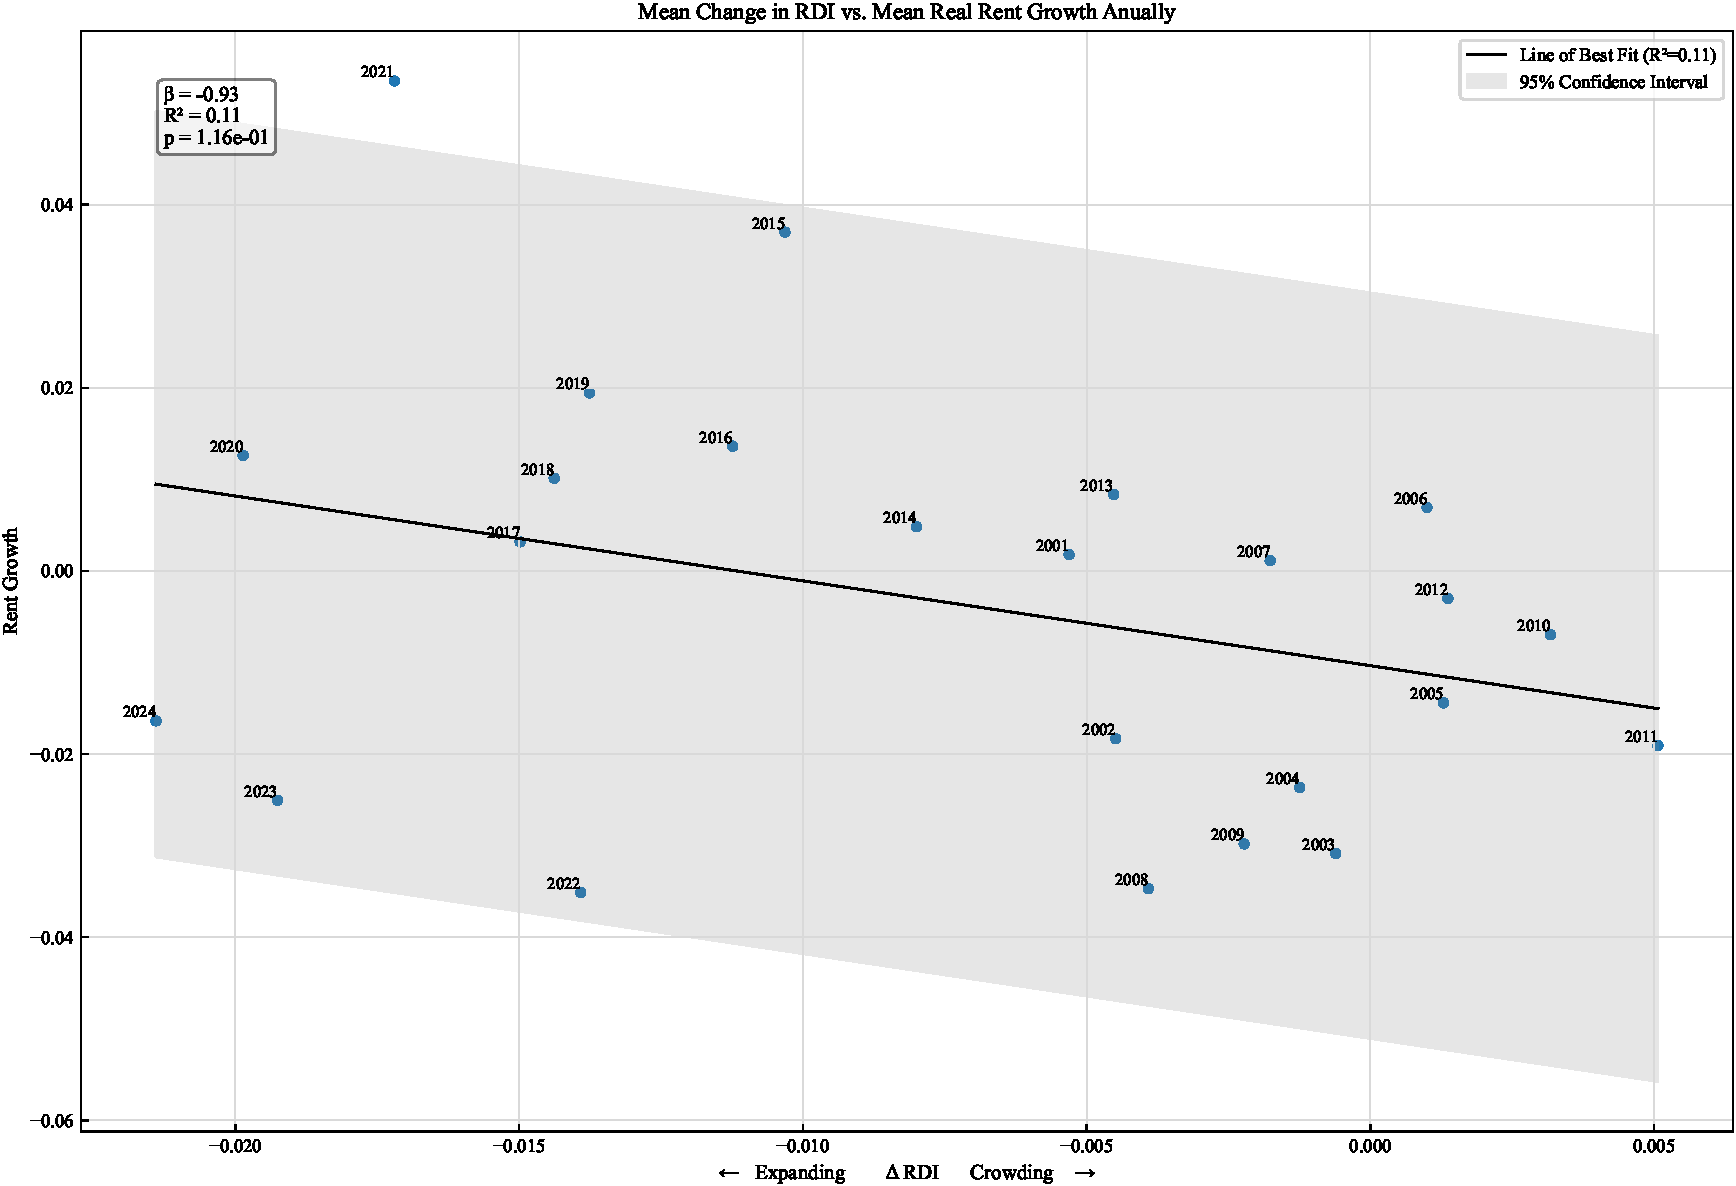
\includegraphics[height=20pc]{rdi_rent_growth_2024.pdf}}
	\caption{Relationship between average annual change in Rental Density Index (horizontal) and average annual relative real rent growth (vertical) in the 100 largest MSAs for each year between 2001 and 2024. \label{fig:rdi_national}}
\end{figure}

Focusing on a panel of the 100 largest metropolitan statistical areas (MSA) between 2000 and 2024, we calculate the RDI. We then examine the year-over-year change in each MSA, in each year. A positive change in RDI (densification) means that population has grown faster than inventory; conversely a negative change in RDI (de-densification) corresponds to inventory growing faster than population. While this ignores the number of households and the percentage of owners versus renters, the signal from the RDI change is robust in spite of this, likely because ownership rates are fairly stationary relative to RDI.

This empirical strategy corresponds with consistent rent growth differences across multiple time horizons. Over the one-year horizon, positive RDI growth  markets significantly outperform negative RDI growth markets. The densifying markets outperform the de-densifying markets by over 100 basis points in real rent growth. The RDI growth also has very strong foresight, with the trailing 10 year changes highly predictive of the next 10 years of supply growth and rent growth. The RDI is especially powerful when analyzed with observed supply growth. It serves as an indicator of when supply will be accretive to rent versus dillutive. In years and markets where the next year's supply exceeds the prior year's RDI growth, real rent growth is significantly below zero. Conversely, when supply is less than the RDI growth, the real rent is significantly greater than zero. These findings suggest that density-based classifications have predictive power and reflect latent demand more accurately than traditional indicators alone.

Our paper makes three principal contributions. First, we introduce the Rental Density Index (RDI), a novel, supply-unbounded metric of housing demand that can be computed at scale from readily available population and unit‐stock data. Second, we show the RDI is a significant indicator of latent demand, using a two-stage least squares model and a very broad panel of foreign in-migration data to measure demand shocks. Finally, we demonstrate RDI’s empirical value using a suite of use-cases applicable to investors, renters, developers, and policy-makers.

These findings carry immediate applications for all housing---market stakeholders. For policymakers, RDI functions as an early-warning gauge of emerging shortages, enabling targeted zoning reforms, calibrated subsidy programs, or expedited permitting in precisely those submarkets under the greatest pressure. Institutional investors and residential developers can embed RDI trends into feasibility and risk models, avoiding the twin hazards of overbuilding in cooling metros or underbuilding in tightening ones. Finally, RDI sharpens the housing‐affordability debate by identifying the locales where rent increases are most likely to outstrip income growth, thereby guiding tenant‐--protection policies, rent‐--assistance programs, and other affordability interventions to the communities that need them most.

In the next section we discuss research on other measures of demand before presenting details on our proposed variable. The Data and Descriptive Statistics section describes and analyzes the density data we used, while the Empirical Strategy section presents evidence and illustrates statistical tests performed to evaluate the validity of the econometric model. In the Forecasting and Validation section, we evaluate the RDI in five different scenarios, showing its power in rent-growth forecasting. The final sections discuss the results of our tests before concluding with implications and further research suggestions. 

\section{Background and Literature Review}
\label{sec2}

A substantial literature in urban and housing economics has sought to measure rental demand using structural modeling, hedonic estimation, and affordability thresholds. Price elasticity estimates, often based on income and housing cost shares, provide insight into how demand responds to price movements under equilibrium assumptions \cite{green2002measuring, malpezzi1996rent}. Hedonic models explain rent levels as a function of unit characteristics and neighborhood amenities, while housing affordability metrics attempt to measure stress via cost-to-income ratios. Though valuable, these approaches often require microdata that are unavailable across time and space or assume frictionless adjustment, limiting their utility in settings with short-run disequilibrium or constrained inventory.

The multifamily housing sector has traditionally relied on indicators such as occupancy rates and net absorption to characterize demand. These measures are intuitive and operationally convenient but are constrained by the size of the existing rental stock. Occupancy, by definition, cannot exceed 100 percent, and absorption is mechanically bounded by the number of new units delivered \cite{mueller1999real, gabriel2001rental}. As a result, such metrics are poorly equipped to detect latent demand, specifically periods in which prospective renters are unable to form households or must cohabitate due to limited supply or rising costs \cite{sirmans1991determinants, pyhrr1999real}. This limitation has become more acute in recent years as algorithmic revenue management systems increasingly target stabilized occupancy thresholds (for example, 95 to 96 percent), further muting variation and diminishing their informational content \cite{calder2024coordinated}.

While these indicators retain short-run forecasting value, they offer limited theoretical insight into renter behavior under constraint. Several studies have documented rent growth during periods of high occupancy but tend to attribute this to restricted supply rather than suppressed household formation \cite{goodman1992rental, wheaton1991realestate}. Structural models, including utility-based choice models \cite{rosenthal1997housing} or equilibrium migration frameworks, provide more detailed behavioral inference but require data on preferences, incomes, or location-specific amenities that are rarely standardized across markets.

Parallel literature in urban economics has studied density, typically defined as people or dwellings per square mile, as a proxy for agglomeration or spatial efficiency. Seminal work by \cite{glaeser2001cities} and \cite{duranton2004micro} links higher density to economic productivity, while more recent studies explore the dual role of densification in shaping housing affordability and urban form \cite{ahlfeldt2019economic, albouy2015driving}. Yet geographic density is primarily a land-use metric; it does not directly reflect household formation or space consumption behavior.

Our work reframes density through a behavioral lens by defining it as the number of people per occupied rental unit: the Rental Density Index (RDI). This metric captures demand pressure more directly than geographic density by tracking how renters adjust their living arrangements under price or supply stress. If renters prefer more space but are observed to cohabitate as rents rise or supply tightens, an increase in RDI reflects a behavioral response to constrained conditions. Conversely, declines in RDI suggest slack: households can afford to spread out. Unlike traditional metrics, RDI growth (\( \Delta \text{RDI} \)) enables analysts to detect crowding pressures even in fully occupied markets.

RDI’s strength lies in its scalability and interpretability. Constructed from widely available data --- population, and rental inventory --- it offers a transparent, repeatable measure of latent demand across markets and over time. This approach is especially valuable in contexts where elasticity models fail to identify pressure due to equilibrium assumptions or unavailable microdata. While elasticity studies estimate how much demand shifts in response to price, RDI captures whether pressure exists at current prices through observed space consumption.

In sum, our contribution is to reinterpret a familiar spatial concept as a dynamic, renter-centered metric that reflects real-time demand conditions. By linking changes in RDI to rent performance, we introduce a new tool for housing market analysis that complements traditional models and offers practical value for forecasting, segmentation, and policy design.

\section{Data and Descriptive Statistics}\label{sec3}
Our market data is sourced from Costar. This includes nominal rent per square foot and rental units by market. Our inflation measures come from the U.S. Bureau of Labor Statistics. And our foreign immigration data at the market level comes from the US Census. We restrict our analysis to the 100 largest U.S. metropolitan statistical areas (MSAs) by multifamily inventory as of 2001, ensuring robust sample representation and consistency over time.

To normalize pricing data across time, we convert all nominal rent figures into real terms using the Consumer Price Index for All Urban Consumers (CPI-U), all-items, provided by the BLS. We convert nominal rent-growth figures into real rent-growth figures by subtracting the annual CPI-U change from the annual rent per square foot change. Although MSA-level inflation indices excluding rent would be ideal, such data are unavailable at a consistent and granular level for our study period. Therefore, real effective rent per square foot and rent growth metrics are adjusted using national CPI. 

Importantly, we standardize rent-growth subtracting each year's median rent growth. We do this to remove the impact of national macroeconomic shocks (i.e., COVID-19). This also serves to stationarize the data and remove the autoregressive tendencies of timeseries data.

Our novel demand variable, the Rental Density Index (RDI), is calculated by dividing population by total rental units at the MSA level. We compute its year-over-year percentage change---\(\Delta\text{RDI}\)---to reflect demand dynamics more accurately. This measure avoids the bounded structure of traditional demand indicators like occupancy and absorption, which are upper bounded by 100\%.

Other variables include supply growth, computed as the quotient of delivered units to the previous year's inventory, and lagged variables prior-year rent growth. 

We exclude New Orleans, LA from our analysis because of its dynamics around the unfortunate aftermath of Hurricane Katrina. Within two years, this MSA had the greatest and least values of RDI growth as well as the greatest and least values of real rent change. 

\begin{table*}[hbt]%
\centering
\caption{Key variables used in the empirical analysis.\label{tab:variables}}%
\begin{tabular*}{\textwidth}{@{\extracolsep\fill}ll@{\extracolsep\fill}}%
\toprule
\textbf{Variable} & \textbf{Description} \\
\midrule
\texttt{CPI}					& Consumer Price Index for All Urban Consumers: All Items in U.S. City Average \\
\texttt{real\_rentpsf}               & Costar's Rent Per Square Foot divided by indexed \texttt{CPI}\\
\texttt{real\_rent\_growth}          & Costar's Effective Rent Growth 12M less Annual percent change in \texttt{CPI} \\
\texttt{relative\_real\_rent\_growth}          & \texttt{real\_rent\_growth} less that year's median \texttt{real\_rent\_growth}\\
\texttt{inventory}             & Existing multifamily rental stock \\
\texttt{delivered}             & Units delivered in the current year \\
\texttt{pop}                   & Total MSA population  \\
\texttt{RDI}			       & Population divided by rental inventory \\
\texttt{delta\_RDI}	           & Yearoveryear percentage change in \texttt{RDI} \\
\texttt{supply\_growth}        & Delivered units divided by the prior year \texttt{inventory} \\
\texttt{foreign\_migration}     & Foreign net migration divided by the area's population \\
\bottomrule
\end{tabular*}
\end{table*}


\subsection{Variable Construction}
The key outcome variable in this study is the \textit{Rental Density Index} (RDI), calculated as the total population divided by the number of rental housing units in a given MSA-year:

\begin{equation*}
	\text{RDI}_{it} = \frac{\text{Population}_{it}}{\text{Rental Units}_{it}}.
\end{equation*}
	
Within the 100 MSAs in the study,this metric ranges from 6.8 to 64.8. It reflects the number of people per rental unit. 
\begin{figure*}[hbt!]
	\centering
	
	\begin{subfigure}[b]{0.32\textwidth}
		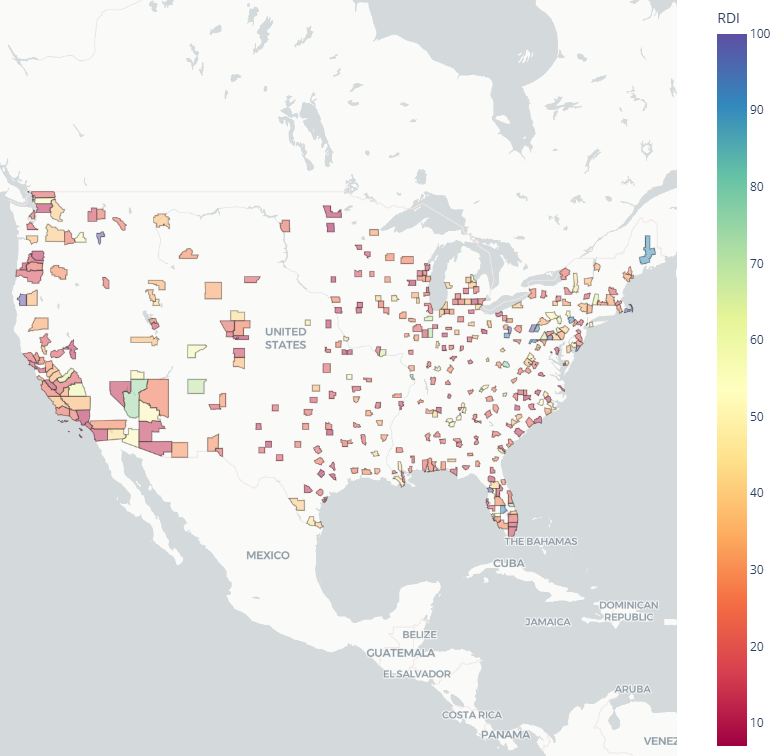
\includegraphics[width=\linewidth]{us.png}
		\caption{United States}\label{fig:us_choropleth}
	\end{subfigure}\hfill
	\begin{subfigure}[b]{0.32\textwidth}
		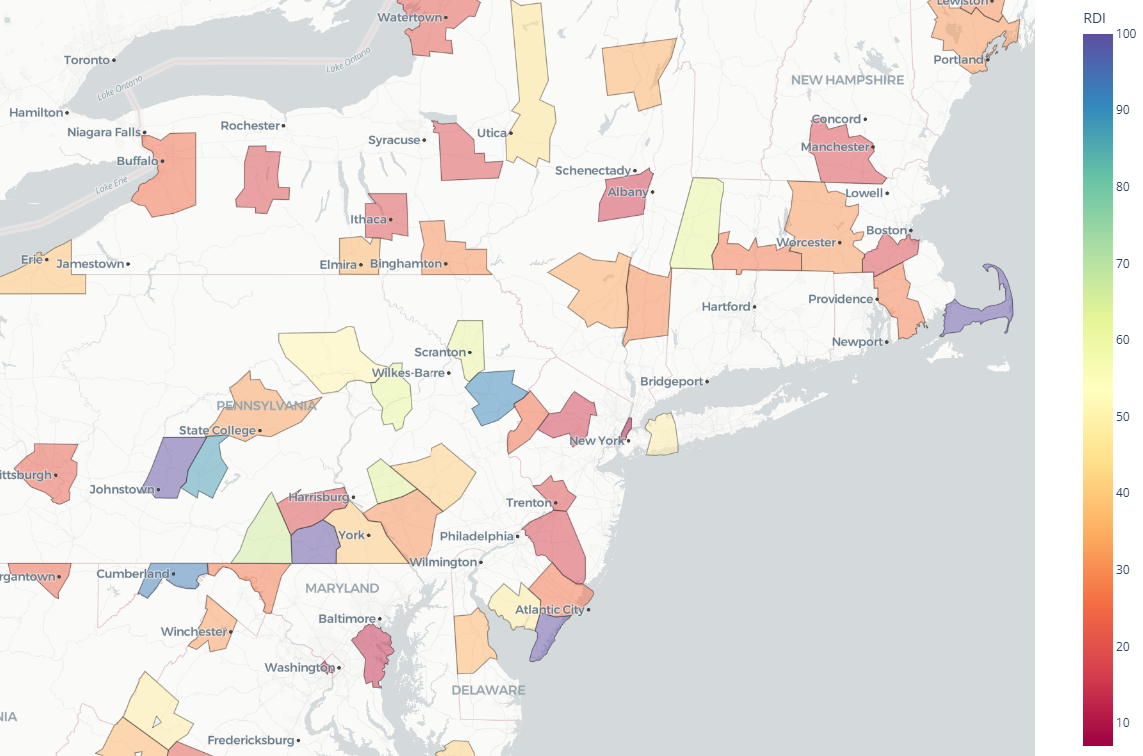
\includegraphics[width=\linewidth]{tristate.png}
		\caption{Tri-State area}\label{fig:tristate_choropleth}
	\end{subfigure}\hfill
	\begin{subfigure}[b]{0.32\textwidth}
		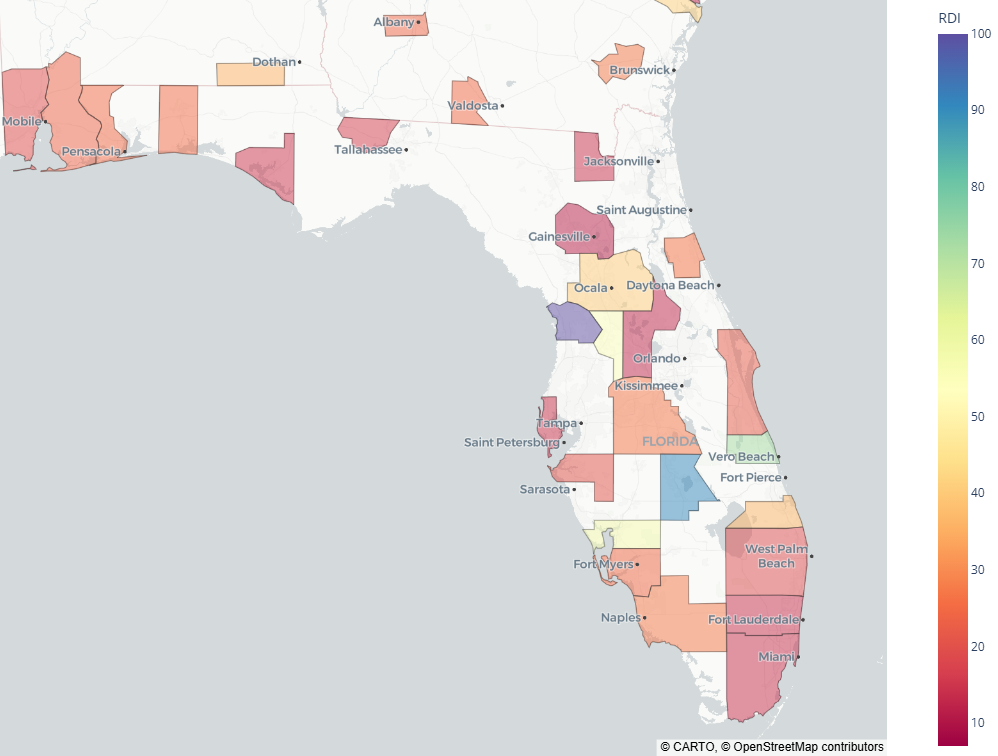
\includegraphics[width=\linewidth]{florida.png}
		\caption{Florida}\label{fig:florida_choropleth}
	\end{subfigure}
	
	\caption{Rental-Density-Index (RDI) choropleths at three spatial scales.}
	\label{fig:choropleth_panel}
\end{figure*}


While the RDI itself is useful for identifying how tight a market is at a given point in time, its absolute level is shaped by long-run demographic and structural trends such as rentership rates and changes in household formation. Accordingly, we focus on the \textit{year-over-year change in RDI}:

\begin{equation*}
	\Delta \text{RDI}_{it} = \text{RDI}_{it} - \text{RDI}_{it-1}.
\end{equation*}


The change in RDI (\( \Delta \text{RDI} \)) offers several advantages. First, it mitigates issues of nonstationarity in the level RDI, enabling cross-market comparison. Second, it reduces the impact of varying rentership percentages across cities. Most importantly, \( \Delta \text{RDI} \) captures demand pressure on housing stock: when it rises, it indicates more people are consolidating into fewer rental units, signaling tightening demand. When it falls, it implies renters are spreading out and absorbing more space, suggesting slack. It is useful to distinguish between two sources of crowding pressure captured by $\Delta \text{RDI}$: price-induced and supply-induced. Price-induced crowding occurs when rising rents outpace incomes, forcing renters to share space or delay household formation---behavioral responses that directly elevate RDI. Supply-induced crowding, by contrast, may arise even without rent escalation if housing stock fails to expand alongside population, resulting in more residents per unit out of sheer constraint. While these mechanisms are observationally similar, our framework implicitly captures both, interpreting $\Delta \text{RDI}$ as the revealed outcome of frictions between housing availability and household spatial preferences. In this way, RDI growth reflects excess demand pressures regardless of whether they arise from affordability shocks or constrained supply.


It is important to note that \(\Delta \text{RDI}\) is conditioned on the rental population and does not explicitly capture shifts between renting and homeownership. Data on home-ownership at the MSA level is sparse, beginning in 2005 and only for the 75 largest MSAs. Furthermore the margins of error are prohibitively large; they are regularly in excess of the annual change percentages and as high as 12.7\% for a single quarter's measurement. Those limitations notwithstanding, the average annual change in homeownership in the largest 75 MSAs from 2015-2024 was 0.20\%, suggesting stationarity. Still, in markets where tenure transitions are volatile---such as during periods of mortgage credit expansion or policy-driven ownership incentives---changes in RDI may partly reflect movement between tenures rather than intra-renter space consumption. For example, a declining RDI could reflect renters exiting into homeownership rather than an easing of rental crowding. While the vast majority of variation in \(\Delta \text{RDI}\) likely reflects household formation and consolidation behavior within the rental market, readers should interpret RDI-based signals with awareness of broader tenure context, especially in markets with known ownership volatility. That said, the average annual change in home ownership is orders of magnitude smaller than either of the RDI components. Between 2002 and 2024 the average annual change in home ownership rate was -0.001, while the average annual change in rental units is 1.35\% and the average annual change in population is 0.75\% over the same time.

\subsection{Summary Statistics}
Table \ref{tab:summary_stats} provides descriptive statistics for the key variables across the full panel. On average, the RDI across all MSAs and years is approximately 18 persons per rental unit, with a standard deviation of 7. The average real rent per square foot is \$0.97, and the average annual growth in rental supply is 1.69\%. The missing records exist only in the beginning or ending years as the prior period and next-period values do not exist. 

\begin{table}[hbt!]
	\centering
	\caption{Summary Statistics}
	\label{tab:summary_stats}
	\begin{tabular}{lrlllllll}
		\toprule
		Unnamed: 0 &  count &      mean &       std &     min &     25\% &       50\% &       75\% &        max \\
		\midrule
		pop &   2500 & 2,010,409 & 2,176,842 & 175,485 & 752,856 & 1,213,619 & 2,422,780 & 14,897,850 \\
		inventory &   2500 &   133,025 &   190,307 &  20,399 &  35,323 &    65,463 &   153,901 &  1,580,435 \\
		supply\_growth &   2400 &      0.02 &      0.02 &   -0.02 &    0.01 &      0.01 &      0.02 &       0.12 \\
		RDI &   2500 &     18.37 &      7.04 &    7.04 &   13.78 &     17.09 &     20.89 &      65.82 \\
		RDI\_growth &   2400 &     -0.01 &      0.01 &    -0.1 &   -0.02 &     -0.01 &       0.0 &       0.04 \\
		real\_rentpsf &   2500 &      0.97 &      0.36 &    0.57 &    0.73 &      0.85 &      1.06 &       2.93 \\
		real\_rent\_growth &   2400 &      -0.0 &      0.03 &   -0.14 &   -0.02 &      -0.0 &      0.01 &        0.2 \\
		\bottomrule
	\end{tabular}
\end{table}




\subsection{Coverage and Representativeness}
The sample includes 2,500 MSA-year observations, covering a mix of large coastal cities, fast-growing Sun Belt metros, and slower-growing Midwestern regions. Together, these MSAs account for over 16 million of the 22 million U.S. apartment units, providing a representative snapshot of national rental dynamics. 

\subsection{Preliminary Observations}

Figure \ref{fig:sidebyside} traces the national Rental Density Index (RDI) from 2000 to 2024. Contrary to conventional wisdom about an acute housing shortage, we observe a steady decline in people per unit (from roughly 16 people-per-unit in 2000 to 13 people-per-unit in 2024). A companion histogram of ΔRDI is stationary but skewed slightly negative, confirming that most years see more units added per new person than vice versa.

\begin{figure}[!htb]
	\centering
	\begin{subfigure}[b]{0.48\textwidth}
		\centering
		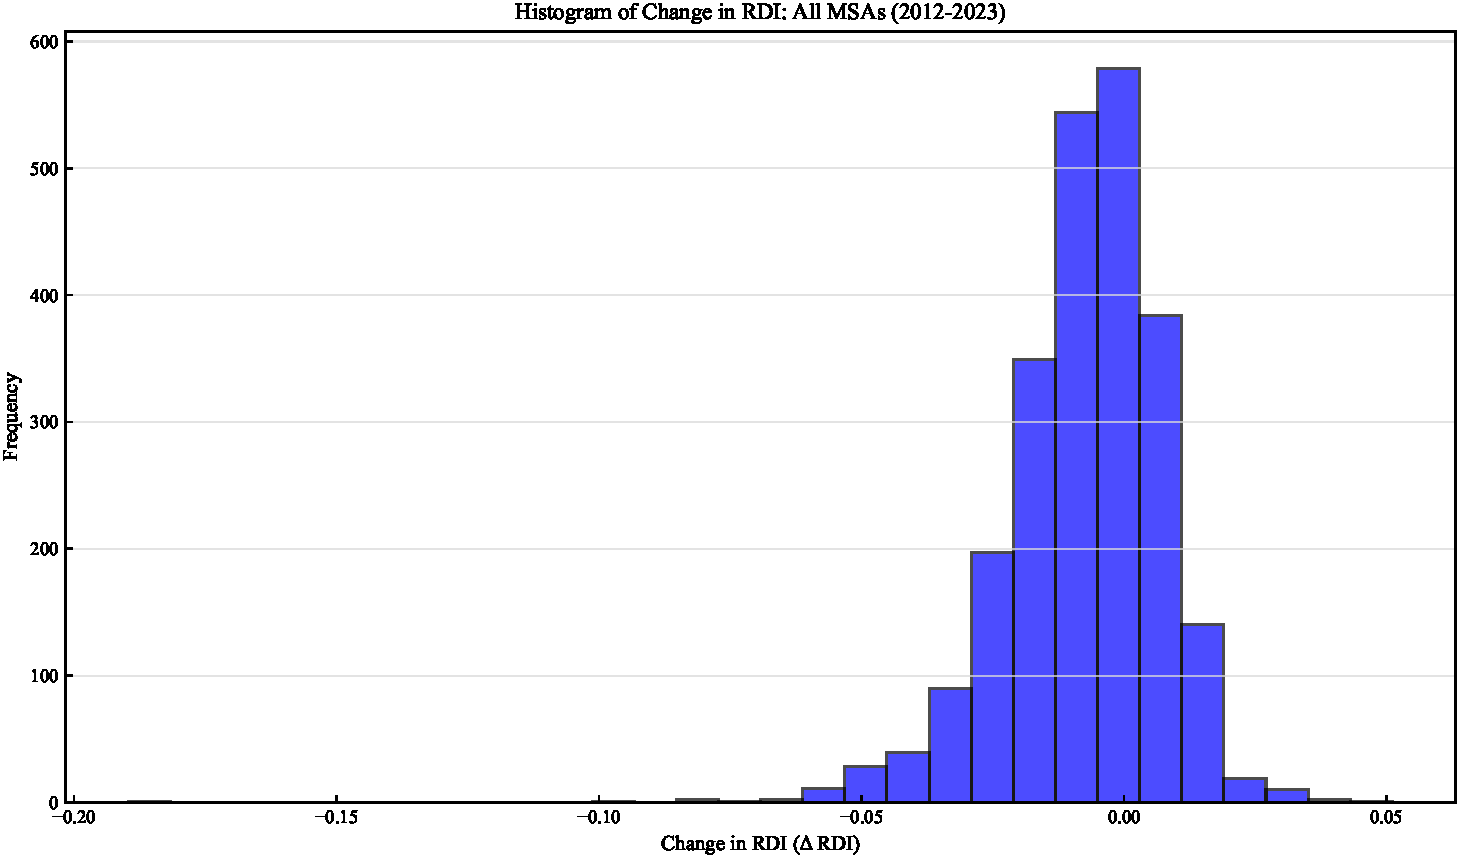
\includegraphics[width=\textwidth]{rdi_growth_histogram.pdf}
		\caption{A histogram of the annual change in RDI across 100 MSAs in the years 2001-2023. The outlier to the left is New  Orleans in 2004, due to Huricane Katrina.\label{fig:rdi_hist}}
	\end{subfigure}
	\hfill
	\begin{subfigure}[b]{0.48\textwidth}
		\centering
		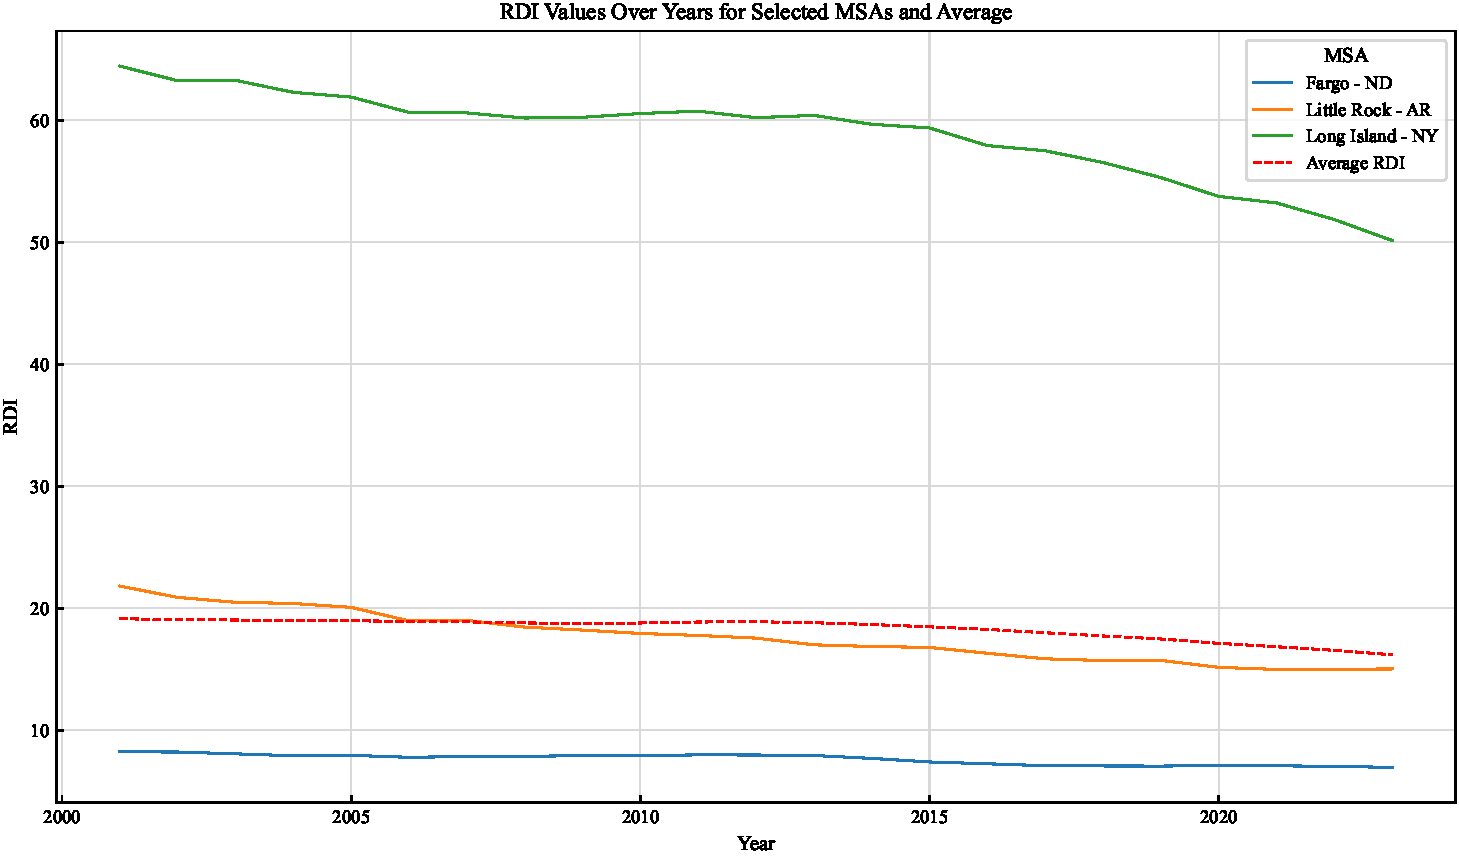
\includegraphics[width=\textwidth]{rdi_trends_selected_msas.pdf}
		\caption{A line graph showing the RDI values (population divided by apartment units) for the MSAs that were the min, max, and median in year 2001}
		\label{fig:rdi_lines}
	\end{subfigure}
	\caption{Histogram of Change in RDI, and Line Graph of RDI}
	\label{fig:sidebyside}
\end{figure}
This pattern illustrates the need for a different demand metric, otherwise the concern for housing shortage seems to be contradicted by a monotonically decreasing housing density. Said differently, occupancy simply reports that units are full--it cannot distinguish whether they are full by choice (everyone prefers roommates) or by necessity (everyone must share). By contrast, year-over-year changes in RDI isolate the relative pace of new people versus new units. In the next section we investigate that property to reveal ΔRDI as a proxy for latent demand. 

\section{Empirical Strategy and Econometric Results}
\label{sec:instrumental-variable}

We estimate the causal effect of crowding, measured as the change in the Rental Density Index (\(\Delta \text{RDI}\)), on future rent growth using a two-stage least squares (2SLS) instrumental variables (IV) approach. This is necessary because \(\Delta \text{RDI}\) may be endogenous to unobserved demand shocks or simultaneous determination with rents. For example, rising rents may compress household formation (raising RDI), or latent shocks could affect both rents and occupancy intensity.

To isolate exogenous variation, we instrument \(\Delta \text{RDI}\) with foreign in-migration as a share of local population, capturing rare and plausibly unanticipated inflows. We implement two instrument definitions: continuous and binary. In the continuous specification, \(\text{exog\_shock}_{it}\) is defined as the year's foreign in-migration as a percent of population. In the binary specification, \(\text{exog\_shock}_{it} = 1\) when foreign in-migration exceeds 0.8\% of population and 0 otherwise. This encompasses approximately 7.2\% of MSA-years and corresponds to a natural break in the distribution of foreign migration. 

To support the validity of these instruments, we confirm that lagged rent growth does not predict foreign in-migration shares. A fixed-effects panel regression of foreign migration share on lagged rent growth yields no significant relationship ($\beta = -0.415$, $p = 0.215$, detailed in Appendix A Section \ref{sec:appendixa}). This result supports the assumption that foreign migration shocks are exogenous with respect to prior local rental market conditions.

The empirical models are specified as follows:
\begin{align*}
	\text{Stage 1:} \quad & \Delta \text{RDI}_{i,t} = \gamma_0 + \gamma_1 \cdot \text{Shock}_{i,t} + \gamma_2 \cdot \mathbf{X}_{i,t} + \mu_i + \delta_t + u_{i,t} \\\\
	\text{Stage 2:} \quad & \text{RentGrowth}_{i,t+1} = \alpha_0 + \beta \cdot \widehat{\Delta \text{RDI}}_{i,t} + \alpha_1 \cdot \mathbf{X}_{i,t} + \mu_i + \delta_t + \varepsilon_{i,t}
\end{align*}
Where:
\begin{itemize}
	\item $\text{RentGrowth}_{i,t+1}$ is next-year relative real rent growth in MSA $i$,
	\item $\Delta \text{RDI}_{i,t}$ is the change in Rental Density Index (crowding pressure),
	\item $\text{Shock}_{i,t}$ is the instrument—either foreign migration share (continuous) or high-migration indicator (binary),
	\item $\mathbf{X}_{i,t}$ includes controls: population growth and sales volume growth,
	\item $\mu_i$ and $\delta_t$ are MSA and year fixed effects.
\end{itemize}


Both specifications (continuous and binary) yield statistically significant and robust estimates. Using the continuous instrument, the estimated effect of \(\Delta \text{RDI}\) is 2.31 (\(p = 0.0010\)), with a strong first-stage F-statistic of 30.3. A placebo test, which replaces the outcome with contemporaneous rent growth, returns a smaller and weaker coefficient (1.66, \(p = 0.0019\)), consistent with a forward-looking interpretation.

Using the binary instrument, the estimated coefficient is 1.68 (\(p = 0.0173\)), with an F-statistic of 39.9. The placebo result remains significant but slightly attenuated (1.61, \(p = 0.0183\)). While the binary version benefits from a cleaner exclusion argument, the continuous specification provides stronger statistical power and supports robustness across specifications.

In contrast, results from lagged instruments are weaker; neither continuous nor binary lagged instruments produce statistically significant estimates, suggesting a contemporaneous relationship between migration shocks and crowding pressure.

\begin{table}[h]
	\centering
	\caption{Summary of 2SLS Estimates of $\Delta \text{RDI}$ on Next-Year Relative Rent Growth for both a Continuous and Binary Shock Variable}
	\label{tab:iv-summary}
	\begin{tabular}{lcccc}
		\toprule
		Instrument Type & Coef. on $\Delta$RDI & Std. Err. & $p$-value & F-stat (1st Stage) \\
		\midrule
		Continuous (contemp.) & 2.31 & 0.70 & 0.0010 & 30.3 \\
		Continuous (placebo)  & 1.66 & 0.53 & 0.0019 & 62.4 \\
		Binary (contemp.)     & 1.68 & 0.71 & 0.0173 & 39.9 \\
		Binary (placebo)      & 1.61 & 0.68 & 0.0183 & 62.9 \\
		Lagged (continuous)   & 1.54 & 0.86 & 0.0740 & 42.8 \\
		Lagged (binary)       & -0.35 & 1.02 & 0.7282 & 62.8 \\
		\bottomrule
	\end{tabular}
\end{table}

Together, these models confirm that exogenous migration shocks produce measurable increases in crowding pressure, and that these crowding effects reliably forecast future rent growth. All specifications include MSA and year fixed effects, ensuring that the estimated relationships are not confounded by time-invariant local characteristics or national-level shocks. The consistency of findings across instrument definitions and robustness checks strengthens confidence in \(\Delta \text{RDI}\) as a causal and timely proxy for rental housing demand.

While the IV model provides a causal estimate of the effect of crowding pressure on rent growth, the subsequent tests in Section ~\ref{forecasting-validation} evaluate whether \(\Delta \text{RDI}\) can serve as a useful predictive signal. These forecasting models do not claim to identify structural relationships, but rather assess the practical value of RDI for anticipating future market conditions.




\section{Forecasting Validation and Real-World Performance}
\label{forecasting-validation}
This section evaluates whether RDI functions as a useful predictive signal for rent growth, independent of causal identification. We organize the analysis into five complementary tests: (1) a simple group-wise ANOVA showing forward rent segmentation by RDI direction; (2) an event study evaluating rent dynamics before and after regime shifts in RDI; (3) a top-vs-bottom quintile spread comparison across forecasting models; (4) a long-horizon signal using count-based RDI persistence; and (5) a diagnostic of supply growth in context, showing how RDI mediates the impact of new supply. Together, these tests examine the predictive performance, durability, and explanatory clarity of RDI across diverse empirical contexts.

\subsection{Predictive Segment Testing: ANOVA on RDI Growth}
We test whether observed changes in RDI can segment markets into meaningful groups in terms of future rent performance. Specifically, we split the samples into two regimes: those with positive $\Delta$RDI and those negative $\Delta$RDI. We then examine whether average next-year relative real rent growth differs significantly across these groups.

Table~\ref{tab:anova-results} shows that markets with positive RDI growth experience average next-year rent growth of 41 basis points above the mean rent growth (significant at p$\leq 3.14^{-14}$), while markets with non-positive RDI growth exhibit an average decline of 15 basis points (significant at p$\leq$0.0026). The difference is statistically significant, as confirmed by both a one-way ANOVA and Tukey’s HSD post-hoc test.

\begin{table}[h]
	\centering
	\caption{ANOVA of Next Year's Relative Real Rent Growth Grouped by RDI}
	\label{tab:anova-results}
	\begin{tabular}{lcccccc} \toprule
		$\Delta$RDI Group & Mean Relative Rent Growth (bps) & SE (bps) & 95\% CI Lower & 95\% CI Upper & $n$ & $p$-value \\ \midrule
		RDI Decline & -15 & 5 & -25 & -5 & 1538 & 0.0026 \\
		RDI Growth & 41 & 7 & 31 & 52 & 762 & $3.14^{-14}$ \\
		\bottomrule
	\end{tabular}
\end{table}

A two-way ANOVA confirms the significance of the group difference ($F = 49.2$, $p \leq 2.98 \times 10^{-12}$), and a Tukey HSD test further validates that the difference in means is statistically distinguishable.
\begin{table}[h]
	\centering
	\caption{Two-Way ANOVA Test Results}
	\label{tab:two-way-anova}
	\begin{tabular}{lcccc} \toprule
		Term & Sum Sq & DF & F & p-value \\ \midrule
		C(demand) & 0.0165 & 1.0 & 49.23 &  $2.98^{-12}$\\
		Residual & 0.7699 & 2298.0 & --- & --- \\
		\bottomrule
	\end{tabular}
\end{table}

\begin{table}[h]
	\centering
	\caption{Tukey HSD Test Results}
	\label{tab:tukey}
	
	\begin{tabular}{lcccccc} \toprule
		Group 1 & Group 2 & Mean Diff & p-adj & Lower & Upper & Reject \\ \midrule
		$\Delta$ RDI $\leq$0 & $\Delta$RDI>0 & 0.0057 & 0.0000 & 0.0041 & 0.0073 & True \\
		\bottomrule
	\end{tabular}
\end{table}

These results show that even without instrumentation, RDI growth serves as a powerful signal for forward rent performance. Practitioners can use RDI segmentation as a lightweight, interpretable classification rule for identifying tight rental markets.

\subsection{Event Study of RDI Regime Transitions}
We next evaluate how rent growth responds dynamically to transitions into and out of RDI-growth regimes. Specifically, we examine rent growth before and after a market switches into a state of positive  $\Delta$RDI (increasing crowding) or  negative  $\Delta$RDI (declining crowding). We continue to examine results in terms of real rent growth relative to the mean rent growth of that year, to avoid capturing rent changes due to macro conditions.

Figure~\ref{fig:event-study} illustrates rent growth over a five-year window centered on the regime switch. The blue line represents transitions into crowding markets, the red line transitions into de-densifying markets, and the gray line shows cases where RDI status does not change.

\begin{figure}[h]
	\centering
	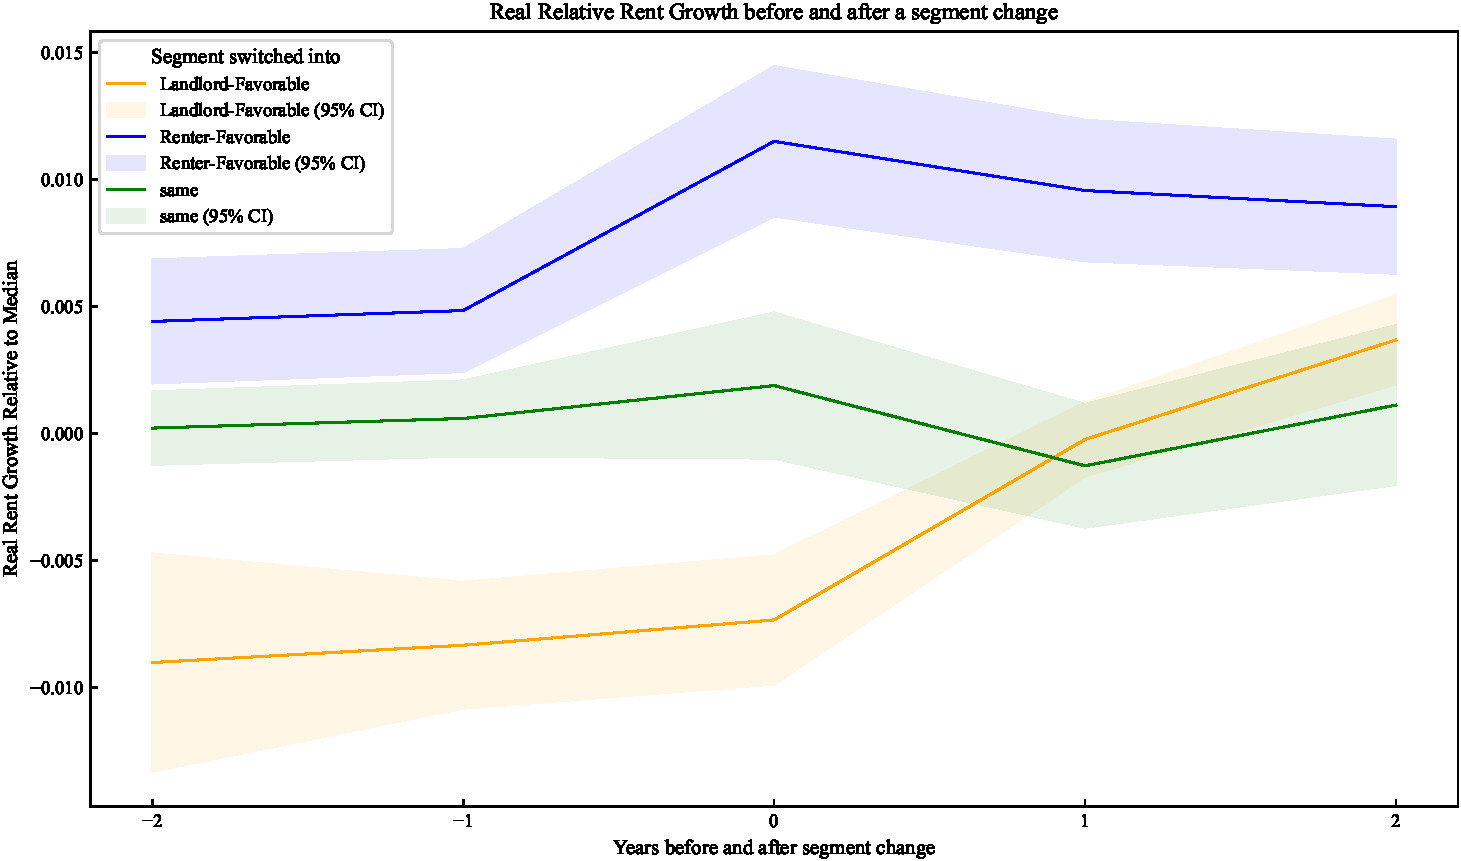
\includegraphics[width=0.8\textwidth]{event_study.pdf}
	\caption{Real Relative Rent Growth Before and After a Market Switches From/To Positive/Negative $\Delta$RDI}
	\label{fig:event-study}
\end{figure}

Table~\ref{tab:event-means} reports differences in average rent growth before and after the regime shift. Markets transitioning into crowded segments see a 48 basis point increase in rent growth, while those exiting see a 29 basis point decline. No significant change is observed when RDI status remains unchanged, as expected.

\begin{table}[h]
	\centering
	\caption{Mean Rent Growth Before and After RDI Regime Transition}
	\label{tab:event-means}
	\begin{tabular}{lcccc} \toprule
		Transition Type & Mean Before & Mean After & Difference & p-value\\ \midrule
		Switched to $\Delta \text{RDI}>0$ & -31 & 17 & 48 & 0.0027\\
		Switched to $\Delta \text{RDI}\leq0$ & 52 & 23 & -29 & 0.0089\\
		No change & -3 & -8 & -5 & 0.6336\\
		\bottomrule
	\end{tabular}
\end{table}

These dynamics confirm that the onset of crowding pressures, as measured by RDI, precedes statistically and economically meaningful changes in rent performance. RDI transitions can therefore serve as timely indicators of shifts in market pricing power.


\subsection{Forecast Spread Comparison: RDI vs ARIMA vs Naïve}
We compare the predictive strength of RDI growth against ARIMA-based and naive trailing average models in forecasting real rent growth across multiple time horizons. For each method, we rank MSAs into quintiles based on their predicted growth and compute the realized top-minus-bottom quintile spread.
Figure~\ref{fig:spread-comparison-quadrant} displays forecast accuracy over one-year, three-year, five-year, and ten-year windows. The RDI-based approach consistently delivers stronger spread segmentation, particularly at longer horizons where traditional time-series methods tend to degrade.

\begin{figure}[h!]
	\centering
	\begin{tabular}{cc}
		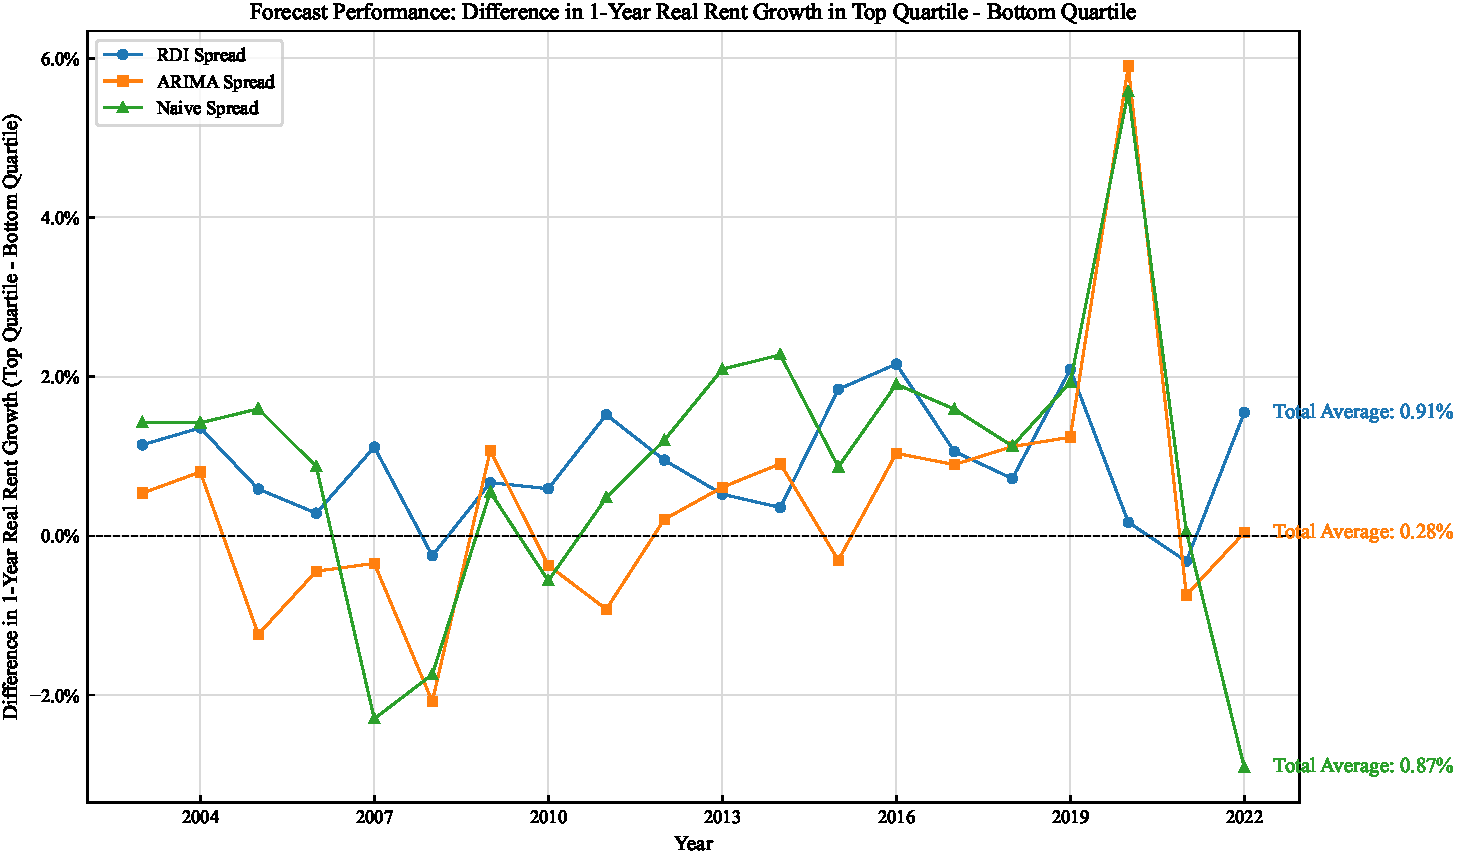
\includegraphics[width=0.45\textwidth]{spread_comparison_over_time_1yr.pdf} &
		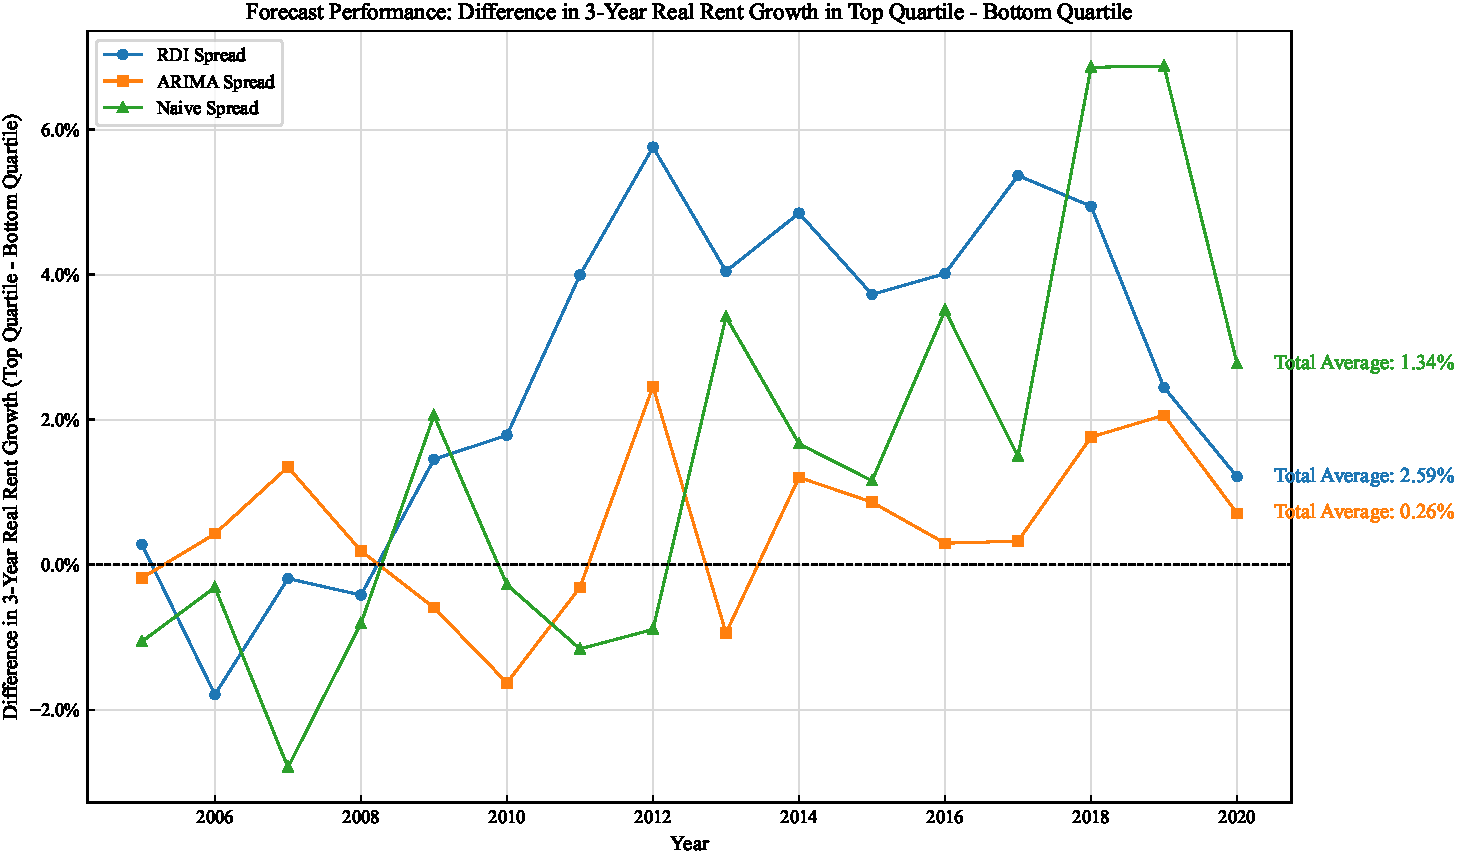
\includegraphics[width=0.45\textwidth]{spread_comparison_over_time_3yr.pdf} \\
		\textbf{(a)} 1-Year Forecast & \textbf{(b)} 3-Year Forecast \\
		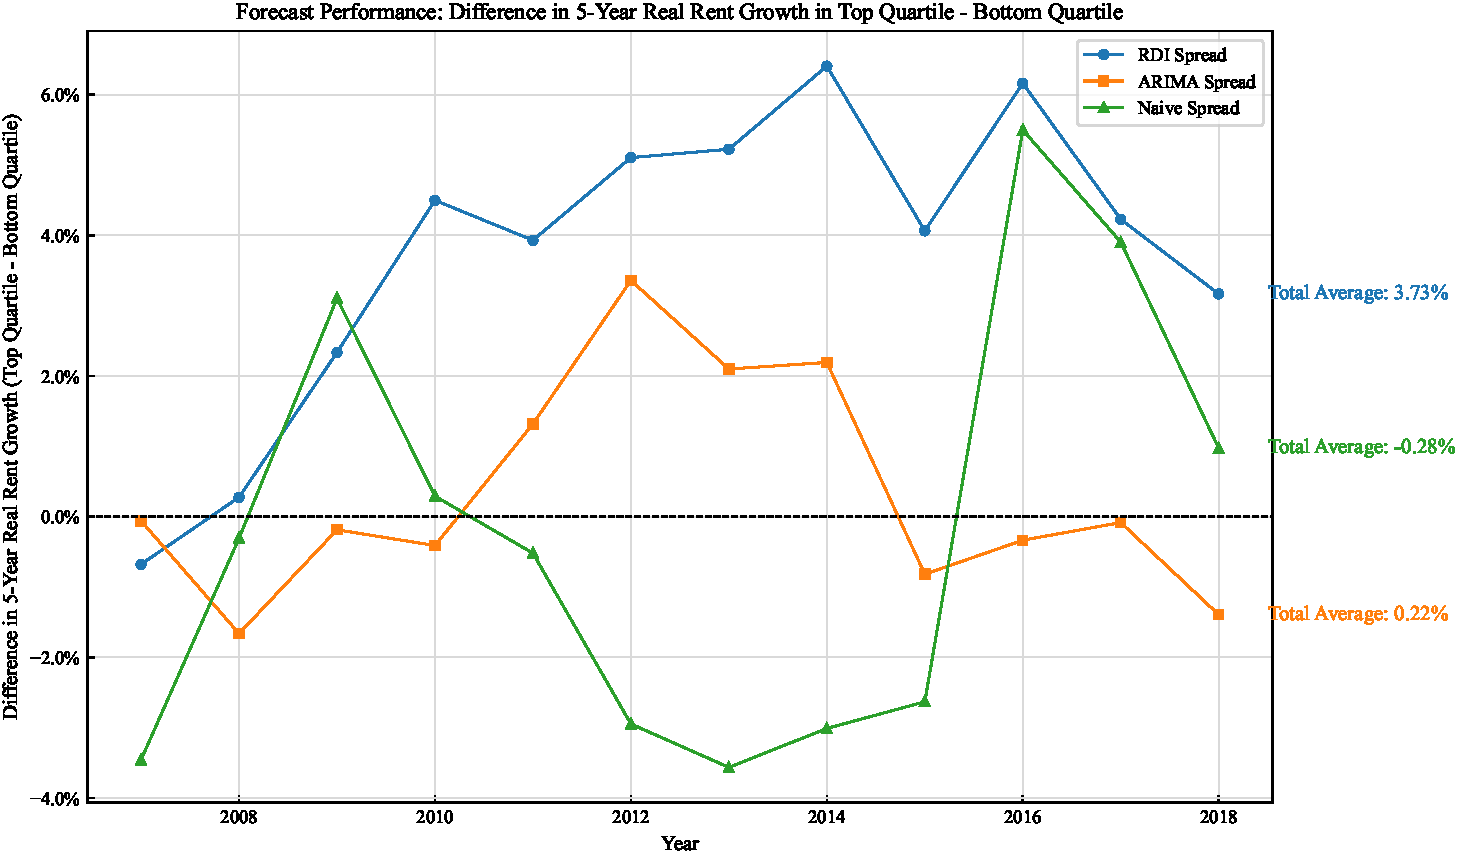
\includegraphics[width=0.45\textwidth]{spread_comparison_over_time_5yr.pdf} &
		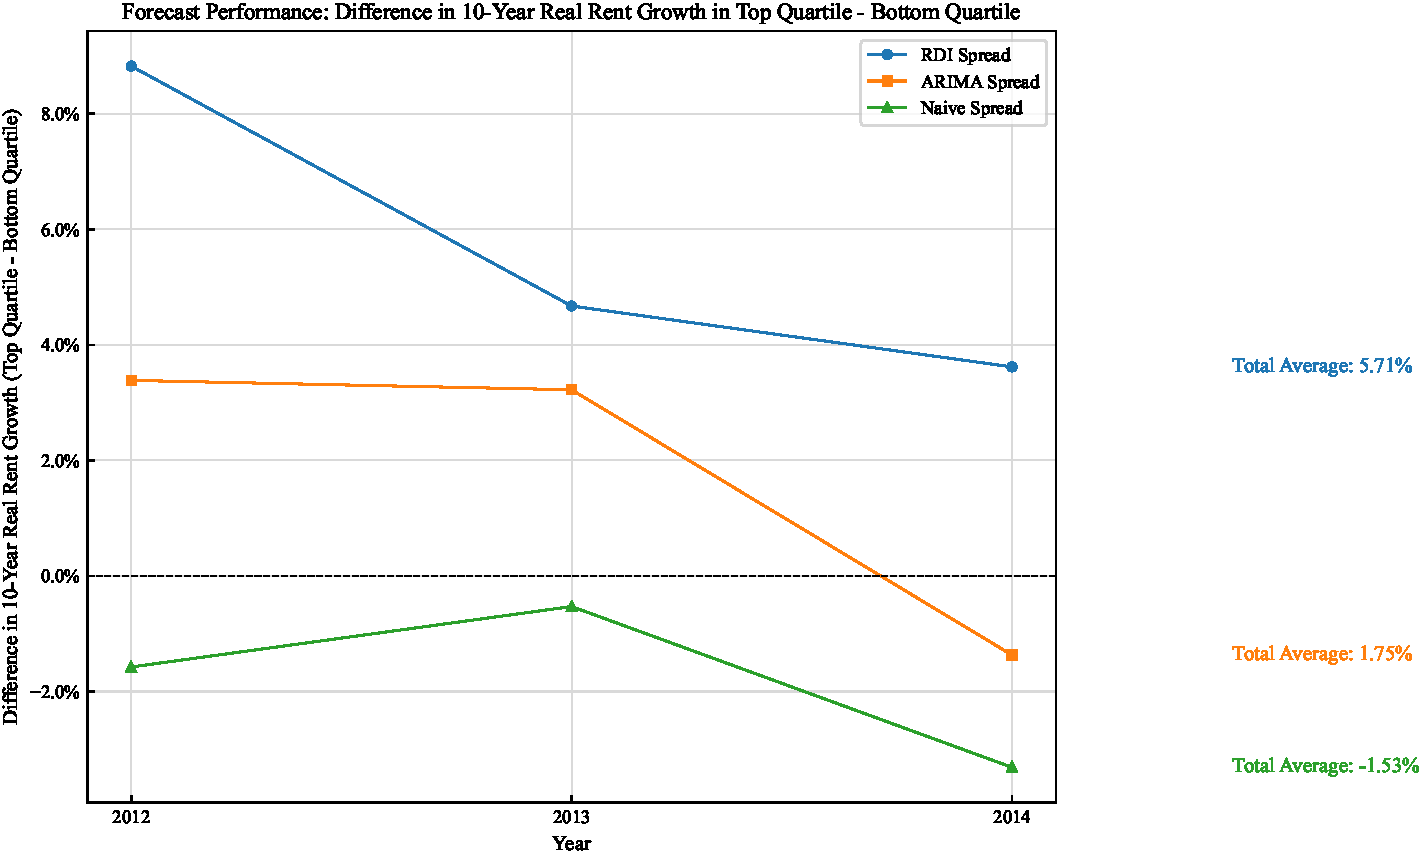
\includegraphics[width=0.45\textwidth]{spread_comparison_over_time_10yr.pdf} \\
		\textbf{(c)} 5-Year Forecast & \textbf{(d)} 10-Year Forecast \\
	\end{tabular}
	\caption{Top-minus-Bottom Quintile Rent Growth Spread by Forecast Method and Horizon}
	\label{fig:spread-comparison-quadrant}
\end{figure}

These results reinforce the value of RDI as a forward-looking predictive signal. Forecasting long-term rent growth is notoriously difficult; most models lose power beyond a few years. That the RDI-based approach maintains signal strength across one-, three-, five-, and ten-year periods underscores its robustness. While time series models rely on trailing trends, RDI captures forward-looking, structural occupancy pressure—making it an effective long-horizon indicator of underlying demand.

\subsection{RDI Positivity Persistence and Long-Term Rent Growth}
We test whether a simple count of trailing years with positive RDI growth serves as a meaningful predictor of future rent appreciation. Specifically, we show the cumulative rent-growth in the following x-years after observing counts of positive RDI growth in the trailing x-years. We look at this over 5 and 10-year rolling periods. 

Figure~\ref{fig:rdi-counts} shows that when n is significantly large, there is a clear, monotonic relationship: markets with more positive RDI observations tend to experience stronger future rent growth. This pattern holds across both time horizons and supports the argument that RDI functions as a persistent, structural signal of housing demand.

\begin{figure}[h]
	\centering
	\begin{tabular}{cc}
		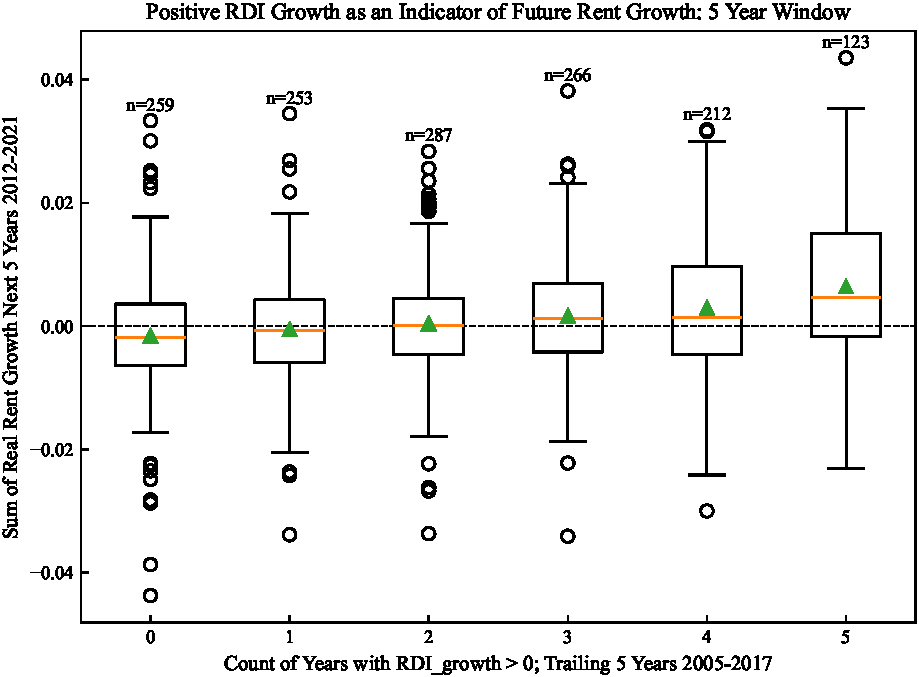
\includegraphics[width=0.45\textwidth]{rdi_positive_counts_vs_rent_growth_5yr.pdf} &
		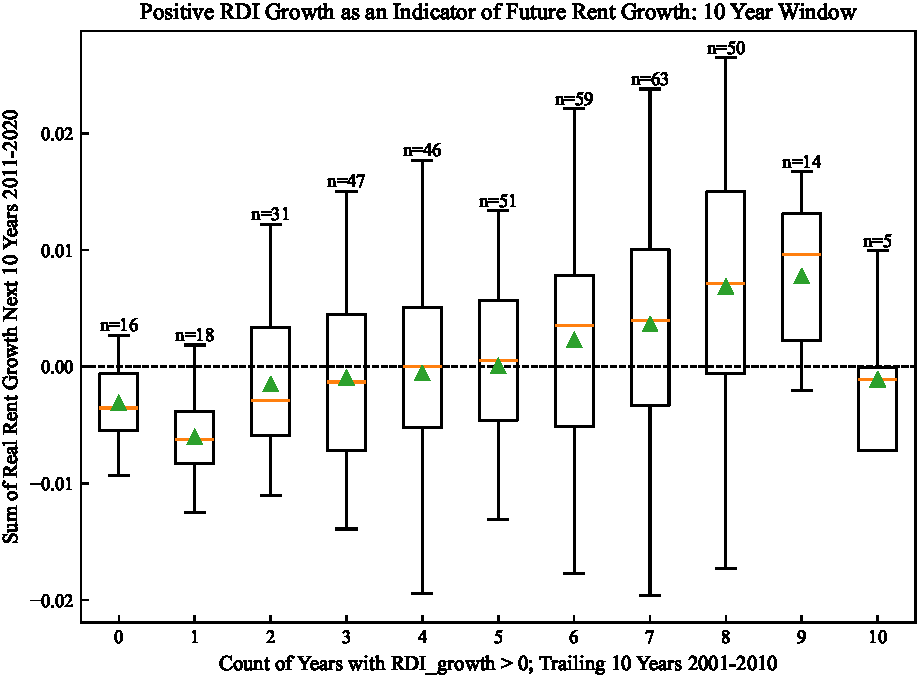
\includegraphics[width=0.45\textwidth]{rdi_positive_counts_vs_rent_growth_10yr.pdf} \\
		\textbf{(a)} 5-Year Horizon & \textbf{(b)} 10-Year Horizon \
	\end{tabular}
	\caption{Cumulative Rent Growth by Number of Positive RDI Years in Prior Window}
	\label{fig:rdi-counts}
\end{figure}

These results reinforce the practical utility of RDI: even without complex forecasting models, the simple count of positive RDI signals---interpreted as consistent crowding pressure---can help classify markets by likely long-term pricing strength.

\subsection{Supply Growth in Context: RDI as a Mediating Lens}
It is often assumed that elevated supply growth should depress rents in subsequent years. To test this assumption, we identify each MSA's year of maximum supply growth and examine the subsequent year’s real relative rent growth. Figure~\ref{fig:supply-growth-rent} shows that the relationship is weak: nearly 45\% of markets still experienced positive rent growth even after their peak supply year, and the overall correlation is low.

In contrast, when we examine how $\Delta$ RDI in those same years (Figure~\ref{fig:supply-growth-rdi}), the relationship between supply growth rent growth is clearer. In markets where supply outstripped population growth the most (farthest left on the X-axis) the rent growth was lowest. Conversely, when supply growth---though at an all-time high--- was closer to population growth, the rents responded more positively. This suggests that crowding pressures, not raw supply levels, capture more of the variance in subsequent rent performance. Even in high-supply environments, strong demand (captured by RDI) can offset what might otherwise appear to be oversupply conditions.

\begin{figure}[h]
	\centering
\begin{subfigure}[b]{0.45\textwidth}
	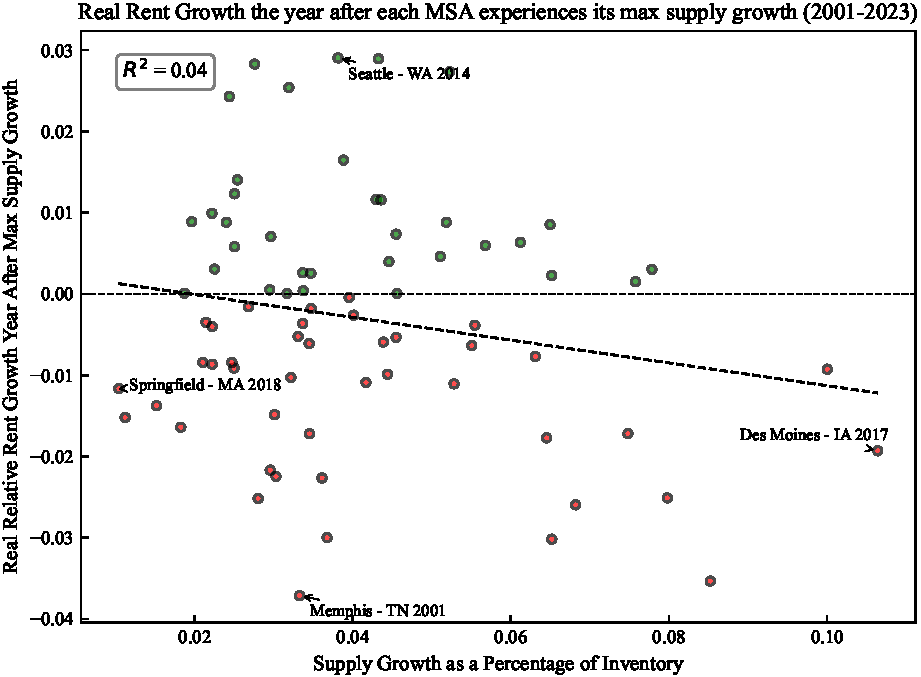
\includegraphics[width=\textwidth]{max_supply_growth_vs_rent_growth.pdf}
	\caption{Supply Growth vs. Subsequent Rent Growth}
	\label{fig:supply-growth-rent}
\end{subfigure}
\hfill
\begin{subfigure}[b]{0.45\textwidth}
	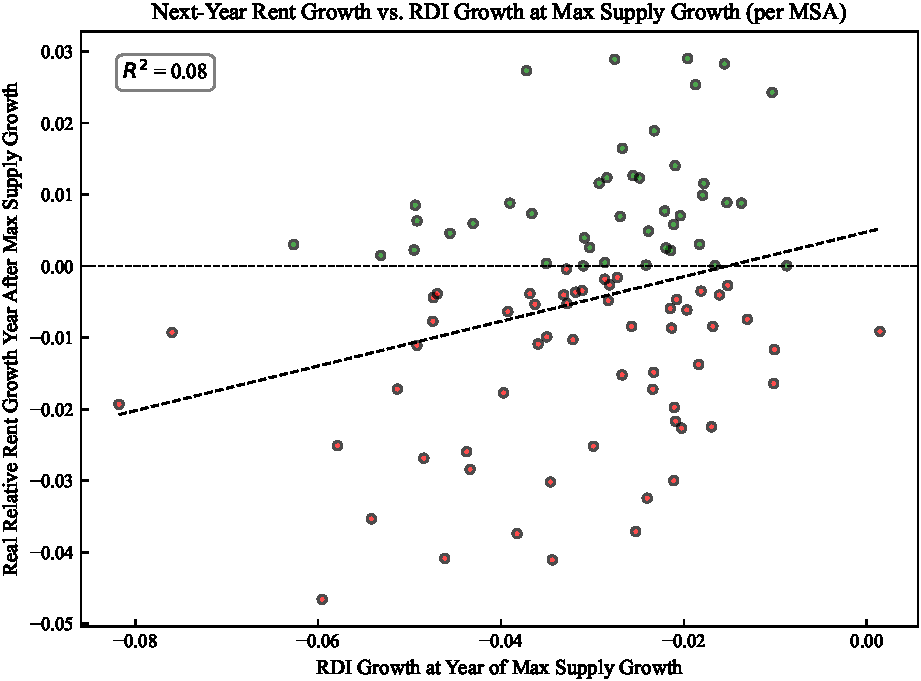
\includegraphics[width=\textwidth]{max_supply_vs_RDI_growth.pdf}
	\caption{Supply Growth vs. RDI Growth}
	\label{fig:supply-growth-rdi}
\end{subfigure}
\caption{Crowding Absorption During Maximum Supply Years}
\label{fig:supply-rent}
\end{figure}
These results challenge the assumption that supply growth alone determines rent dynamics. Without considering how supply is absorbed relative to household formation, analysts risk misclassifying healthy markets as oversupplied. RDI offers a more reliable, demand-sensitive lens.

\subsection{Summary: RDI as a Practically Useful, Predictively Durable Demand Metric}
The empirical tests in this section demonstrate that RDI---a simple, observable measure of household crowding---delivers meaningful insight into rental market behavior. Across multiple frameworks, RDI consistently outperforms: it segments markets with forward---looking rent divergence, anticipates regime transitions, and reveals demand absorption dynamics even during peak supply years.

These results complement the causal identification strategy in Section~\ref{sec:instrumental-variable}, where instrumented RDI growth was shown to drive future rent increases. Here, we show that RDI also performs well in practice without instrumentation, making it suitable for real-time forecasting, benchmarking, and investment decisions.

While RDI is not without limits---its precision may weaken in data-sparse MSAs or highly regulated rent environments---it stands out as a behaviorally grounded, interpretable, and statistically durable signal of latent housing demand.


\section{Discussion}
This paper demonstrates that crowding pressure, as measured by changes in the Rental Density Index, serves as a robust and forward-looking indicator of rental market tightness. Our empirical analyses show that \(\Delta\text{RDI}\) reliably predicts future rent growth, highlighting the hidden intensity of rental housing demand even when traditional market metrics such as occupancy rates remain stable. By distinguishing between the causal role of \(\Delta\text{RDI}\) in driving rent growth and its practical forecasting utility, we establish the broad applicability and effectiveness of this indicator. The findings underscore the versatility of \(\Delta\text{RDI}\) as both a rigorous economic indicator of underlying market dynamics and a practical forecasting tool for diverse market participants.

\subsection{Advantages}
Unlike traditional, static metrics such as occupancy and absorption, \(\Delta\text{RDI}\) dynamically captures behavioral adjustments by households responding to housing constraints, such as increased roommate formation or delayed household formation. These early behavioral signals often precede rent increases, positioning \(\Delta\text{RDI}\) as a valuable leading indicator.

Significantly, \(\Delta\text{RDI}\) retains predictive strength across various forecasting horizons, consistently outperforming traditional ARIMA and naive trailing-average models, even in out-of-sample tests. Its predictive accuracy, particularly notable in forecasting rent trends over longer periods (such as ten-year horizons), underscores its robustness and practical applicability.

The clear implications for policy-makers, investors, and renters make \(\Delta\text{RDI}\) particularly valuable. For policymakers, it offers an early warning signal of emerging housing shortages or surpluses, facilitating timely and targeted interventions such as zoning reforms, targeted subsidies, and expedited permitting processes. Investors and developers can integrate \(\Delta\text{RDI}\) into their risk management and feasibility analyses, enhancing strategic decisions about market entry, asset allocation, and development timing. Renters benefit from clearer market signals about impending rent increases, enabling better-informed housing decisions and advocacy efforts. Thus, \(\Delta\text{RDI}\) provides a structurally sound, scalable, and practical framework for anticipating and managing market dynamics across multiple contexts.

\subsection{Limitations: Tenure Shifts and Spatial Spillovers}

While \(\Delta\text{RDI}\) offers a parsimonious and scalable indicator of rental demand pressure, it is important to acknowledge two interpretive limitations. First, the framework assumes a stable tenure composition—i.e., that observed changes in population per occupied rental unit reflect shifts within the renter segment. However, in some markets, changes in RDI may be partially driven by tenure transitions, such as households moving into homeownership or into rental units from ownership due to credit constraints or housing cost burdens. For example, a declining RDI might suggest easing crowding pressure, but could also reflect renter outmigration into the owner-occupied segment. Conversely, increasing RDI may reflect ownership lock-in effects or affordability barriers that delay household formation. While these effects likely operate at the margin in most MSAs, acknowledging tenure fluidity is important for fully interpreting RDI-based signals. Future work could extend the RDI framework by incorporating tenure transition data or endogenizing homeownership trends.

Second, the current analysis treats each metropolitan statistical area (MSA) as an independent unit. In practice, however, housing market conditions are rarely contained by administrative boundaries. Migration, affordability spillovers, and commuting patterns often link neighboring MSAs, meaning that crowding pressures in one region may affect rental markets in adjacent areas. Ignoring these spillover dynamics may understate the correlated nature of demand shifts, especially in highly integrated urban corridors. Incorporating spatial dependence structures or spatially lagged RDI variables in future work may enhance model precision and improve detection of regional displacement or diffusion effects.

While we do not formally estimate a spatial lag model, we assess geographic clustering by examining pairwise correlations in $\Delta \text{RDI}$ across neighboring MSAs. We find strong co-movement among regionally linked markets—e.g., New York and Northern New Jersey ($r = 0.70$), San Francisco and San Jose ($r = 0.69$), and Dallas–Fort Worth and Austin ($r = 0.77$). More details can be found in Appendix B. These results suggest that crowding pressures often evolve in tandem across proximate metros, reflecting regional migration flows, shared housing constraints, or price spillovers. Future work could formalize these relationships using spatial dependence structures or migration-network adjacency matrices.

\section{Conclusion}

We propose the Rental Density Index (RDI) as a demand-centric metric for measuring latent pressure in multifamily rental markets. By tracking changes in population per occupied unit, RDI captures household-level crowding dynamics that precede and predict future rent movement. Our empirical results, validated across causal models, forecasting tests, and event studies, establish (\(\Delta\text{RDI}\)) as both a leading indicator and a practical classification tool.

The simplicity of RDI is a strength. While traditional demand estimation often requires detailed demographic or income data, RDI can be computed with widely available population and housing stock data. Yet it performs comparably—if not better—than more complex models, especially over long forecast horizons. It is also behaviorally grounded: renters adjust space usage when pricing becomes constrained, and this adjustment leaves measurable traces in the data.

Future research may extend this work in several directions. RDI could be evaluated alongside migration flows, income segmentation, or micro-level leasing data to refine its predictive specificity. It may also prove useful in pricing models, rent control policy evaluation, or early-warning systems for affordability crises.

In sum, this paper offers both a new way to quantify housing demand and a practical framework for translating that signal into market insight. (\(\Delta\text{RDI}\)) helps bridge the gap between structural economics and applied decision-making—and in doing so, offers analysts, policymakers, and investors a grounded, interpretable, and scalable tool for anticipating market behavior.

\section*{Appendix A: Instrument Validity}
\label{sec:appendixa}

To assess the exogeneity of our instrument, we test whether lagged relative rent growth predicts the share of foreign in-migration. We estimate:

\[
\text{foreign\_migration\_share}_{i,t} = \alpha + \beta \cdot \text{RentGrowth}_{i,t-1} + \gamma \cdot \textbf{X}_{i,t} + \mu_i + \delta_t + \varepsilon_{i,t}
\]

where $\textbf{X}_{i,t}$ includes population growth and sales volume growth, and $\mu_i$ and $\delta_t$ represent MSA and year fixed effects. The coefficient on lagged rent growth is statistically insignificant ($\beta = -0.415$, $p = 0.215$), providing support for the orthogonality of foreign migration shocks to prior local rent conditions.
\section*{Appendix B: Spillover Effect Correlation Matrix}
\begin{table}[h]
	\centering
	\caption{Cross-MSA Correlation in $\Delta \text{RDI}$ Among Regional Pairs}
	\label{tab:regional_corr}
	\begin{tabular}{lcc}
		\toprule
		MSA 1 & MSA 2 & Correlation ($r$) \\
		\midrule
		New York, NY & Northern New Jersey, NJ & 0.70 \\
		San Francisco, CA & San Jose, CA & 0.69 \\
		Dallas–Fort Worth, TX & Austin, TX & 0.77 \\
		Los Angeles, CA & Inland Empire, CA & 0.52 \\
		Miami, FL & Palm Beach, FL & 0.54 \\
		\bottomrule
	\end{tabular}
\end{table}


%\backmatter
\bmsection*{Author contributions}

All authors contributed equally

\bmsection*{Acknowledgments}


\bmsection*{Financial disclosure}

\bmsection*{Conflict of interest}


\bmsection*{Data Disclosure}


\bibliography{wileyNJD-APA}
\bmsection*{Supporting information}

Additional supporting information may be found in the
online version of the article at the publisher’s website.










\nocite{*}% Show all bib entries - both cited and uncited; comment this line to view only cited bib entries;


\end{document}
